\documentclass[11pt]{article}
\usepackage[ngerman]{babel}

\usepackage{amsmath,amssymb, a4, verbatim}
%\usepackage[latin1]{inputenc}
\usepackage[utf8]{inputenc} % üöäß
\usepackage{listings} % für inline codelistings
\lstset{%
		basicstyle=\ttfamily,		% the size of the fonts
		columns=fixed,				% anything else is horrifying
		showspaces=false,				% show spaces using underscores?
		showstringspaces=false,		% underline spaces within strings?
		showtabs=false,				% show tabs within strings?
		xleftmargin=1.5em,				% left margin space
}
\lstdefinestyle{inline}{basicstyle=\ttfamily}
\newcommand{\listline}[1]{\lstinline[style=inline]!#1!}

\usepackage{caption}
\newcommand{\tinycaption}[1]{\captionsetup{labelformat=empty}\caption{#1}}

%\usepackage{color}
%\usepackage{epsfig} % eps
\usepackage{graphicx} % eps
%\usepackage[shortcuts]{extdash}
%\usepackage{dsfont}
%\usepackage{epstopdf} % eps
%\usepackage[pdf]{pstricks} % eps
%\usepackage{auto-pst-pdf}
\usepackage{mathtools}
\usepackage{dsfont} % $ \mathds{1} $
\usepackage{icomma}
\usepackage{tikz}
%\usepackage{pgfplots}

%\pgfplotsset{compat=1.8}
\usepackage[bottom]{footmisc} % put footnotes at the bottom of page
\usepackage{nicefrac} % für brüche die aussehen wie prozentzeichen
% \usepackage{ps2pdf}
\usetikzlibrary{automata,positioning}

\usepackage{algorithmicx}
\usepackage{algpseudocode}
\usepackage{algorithm}

\usepackage{multicol}
\setlength{\columnseprule}{0.5pt}
\def\columnseprulecolor{\color{black}}
\usepackage{wrapfig} % make stuff float
\usepackage{placeins} % stop stuff from floating
\usepackage{seqsplit} % very long numbers
\usepackage{framed} % begin{framed}

%	Headings and Footings :
\usepackage{fancyhdr}
\headheight15pt
\headsep1pt
\footskip22pt
\lhead{Technische Mechanik II, \ueberschrift}

\chead{}
\usepackage{lastpage}
\rhead{Seite \thepage~von \pageref{LastPage}}
\renewcommand{\headrulewidth}{.4pt}

\usepackage[yyyymmdd]{datetime}
\renewcommand{\dateseparator}{--}
\lfoot{\today}
\cfoot{}
\rfoot{Joshua}
\renewcommand{\footrulewidth}{.4pt}

%----------------------------------------------------------------

% https://tex.stackexchange.com/questions/54492/change-the-bottom-and-top-margin-of-section-and-subsection
\usepackage[compact]{titlesec}

% Spacing corresponding to `book` class
% \titlespacing*{\section} {0pt}{3.5ex plus 1ex minus .2ex}{2.3ex plus .2ex}
% \titlespacing*{\subsection} {0pt}{3.25ex plus 1ex minus .2ex}{1.5ex plus .2ex}

% Spacing before/after reduced by 1ex each
\titlespacing*{\section}       {0pt}{0.5ex  plus 0ex minus 0.5ex }{0.3ex plus 0ex minus 0.3ex}
\titlespacing*{\subsection}    {0pt}{0.25ex plus 0ex minus 0.25ex}{0.2ex plus 0ex minus 0.2ex}
\titlespacing*{\subsubsection} {0pt}{0.25ex plus 0ex minus 0.25ex}{0.2ex plus 0ex minus 0.2ex}

\textwidth16.5cm
\oddsidemargin0.cm
\evensidemargin0.cm

\def\somedistanceTop{1.1cm}
\def\somedistanceLeft{.5cm}

\usepackage[]{geometry}
\geometry{
	a3paper, %landscape,
	%	total={170mm,257mm},
	left=\somedistanceLeft,
	right=\somedistanceLeft,
	top=\somedistanceTop,
	bottom=\somedistanceTop
}

\parindent0cm

\newcommand{\R}{ {\mathbb R} }
\newcommand{\C}{ {\mathbb C} }
\newcommand{\1}{ {\mathds{1}} }
\newcommand{\abs}[1]{\lvert#1\rvert}
\newcommand{\norm}[1]{\left\lVert#1\right\rVert}
\newcommand{\xt}{\tilde{x}}
\newcommand{\dotleq}{\dot{\leq}}
\newcommand{\m}{\hphantom{-} }

\newcommand{\dashfill}[1]{\vspace{11pt}\def\dashfill{\cleaders\hbox{#1}\hfill}\hbox to \hsize{\dashfill\hfil}\vspace{11pt}}
\newcommand{\scdot}{\!\cdot\!}

\newcommand{\sig}{\text{signum}}
\newcommand{\rot}{}

% ------------------	edit Ueberschrift ---------------------
\newcommand{\ueberschrift}{TM II Formeln}

\usepackage{mathtools}
\usepackage{ragged2e}
\newlength\ubwidth
\newlength\obwidth
\newcommand\underbraceWrap[3][0pt]
{
	\settowidth\ubwidth{$#1$}
	\underbrace{#2}_
	{
		\parbox
		{
			\maxof{\ubwidth}{\numexpr#1}
		}
		{
			\scriptsize\Centering#3
		}
	}
}
\newcommand\overbraceWrap[3][0pt]
{
	\settowidth\obwidth{$#1$}
	\overbrace{#2}^
	{
		\parbox
		{
			\maxof{\obwidth}{\numexpr#1}
		}
		{
			\scriptsize\Centering#3
		}
	}
}

%for use in \int
\newcommand{\td}{\,\text{d}}

\input{tex/greek.tex}

\setcounter{secnumdepth}{5}
\setcounter{tocdepth}{5}

% for clickabe stuffs
\usepackage{hyperref}
\hypersetup{
	colorlinks,
	citecolor=black,
	filecolor=black,
	linkcolor=black,
	urlcolor=black
}

\usepackage{empheq}
\usepackage{soul}
\usepackage{xcolor}

\usepackage{framed}
\setlength\FrameSep{0.5em}
\setlength\OuterFrameSep{\partopsep}

% https://tex.stackexchange.com/questions/6812/an-environment-to-change-the-vertical-space-around-a-formula
\newenvironment{shrinkeq}[1][-0ex]
{\bgroup
	\addtolength\abovedisplayshortskip{#1}
	\addtolength\abovedisplayskip{#1}
	\addtolength\belowdisplayshortskip{#1}
	\addtolength\belowdisplayskip{#1} \[}
{\]\egroup\ignorespacesafterend}

\usepackage{varwidth}
\newcommand{\umrandet}[1]{\pbox{\textwidth}{\boxed{\text{#1}}}}

% https://tex.stackexchange.com/questions/112576/math-mode-in-tabular-without-having-to-use-everywhere
\usepackage{amstext} % for \text macro
\usepackage{array}   % for \newcolumntype macro
\newcolumntype{L}{>{$}l<{$}} % math-mode version of "l" column type

\setlength{\fboxsep}{0pt}
\usepackage{environ}
\NewEnviron{formel}[2][white] % green!60!white!50
{
%	\setlength\FrameSep{\fboxsep}
%	\begin{framed}\noindent%
	\colorbox{#1}{
		\parbox{1.0\linewidth-7.3pt}
		{
			\begin{shrinkeq}
				\boxed{
					\tag{#2}
					\begin{split}
						\BODY
					\end{split}
				}
			\end{shrinkeq}
		}
	}
%	\end{framed}
}
\NewEnviron{formelAt}[3][white] % green!60!white!50
{
%	\setlength\FrameSep{\fboxsep}
%	\begin{framed}\noindent%
	\colorbox{#1}{
		\parbox{1.0\linewidth-7.3pt}
		{
			\begin{shrinkeq}
				\boxed{
					\tag{#2}
					\begin{alignat}{#3}
						\BODY
					\end{alignat}
				}
			\end{shrinkeq}
		}
	}
%	\end{framed}
}

%\usepackage{showframe}
% -----------------------------------------------------------
\begin{document}
		\abovedisplayskip = 2pt plus 0pt minus 2pt
		\belowdisplayskip = 2pt plus 0pt minus 2pt
		\abovedisplayshortskip = 2pt plus 0pt minus 2pt
		\belowdisplayshortskip = 2pt plus 0pt minus 2pt

		\pagestyle{fancy}

%	\begin{multicols*}{3}
%		\pagenumbering{roman}
%		\tableofcontents
%	\end{multicols*}
%	\pagebreak
	\pagenumbering{arabic}

	\begin{multicols}{3}

		\section{Zug und Druck in Stäben}
		\subsection{Spannung} % 1.1
		
		\begin{formel}{1.1}
			\underbrace{\sigma}_{\text{Spannung}\left[\frac{N}{mm^2}\right]}
			=
			\frac{\overbrace{N}^{\text{Normalspannung}\left[N\right]}}{\underbrace{A}_{\text{Fläche}\left[mm^2\right]}}
		\end{formel}
		\begin{formel}{1.2}
			\underbrace{\sigma}_{\text{Spannung}\left[\frac{N}{mm^2}\right]}
			=
			\frac{\overbrace{F}^{\text{Kraft}\left[N\right]}}{\underbrace{A}_{\text{Fläche}\left[mm^2\right]}}
		\end{formel}
		\begin{formel}{1.3}
			\sigma
			=
			\frac{\overbraceWrap[95pt]{\sigma_0 = \nicefrac{F}{A}}{Normalspannung in einem Schnitt Senkrecht zur Stabachse}}{2}
			\left(1 + \cos 2 \varphi\right)
			,&
			\tau
			=
			\frac{\sigma_0}{2}
			\left(\sin 2 \varphi\right)
		\end{formel}
		\begin{formel}[green!60!white!50]{1.4}
			\sigma(x)
			=
			\frac{N(x)}{A(x)}
		\end{formel}
		\begin{formel}[green!60!white!50]{1.5}
			A_{\text{erf}}
			=
			\frac{\abs{N}}{\sigma_{\text{zul}}}
		\end{formel}

		\subsection{Dehnung} % 1.2

		\begin{formel}[green!60!white!50]{1.6}
			\underbrace{\varepsilon}_{\text{Dehnung} \left[1\right]} 
			=
			\frac{\overbrace{\Delta \ell}^{\text{Verlängerung}\left[m\right]}}
					 {\underbraceWrap[50pt]{\ell_0}{Ursprüngliche Länge $\left[m\right]$}}
			=
			\frac{\ell - \ell_0}{\ell_0}
		\end{formel}

		Örtliche (lokale Dehnung)

		\begin{formel}[green!60!white!50]{1.7}
			\varepsilon(x)
			=
			\frac{\text{d}u}{\text{d}x}, \quad \abs{\epsilon} \ll 1
		\end{formel}

		\subsection{Stoffgesetz}

		Hooke'sches Gesetz \\
		\nopagebreak
		\begin{formel}[green!60!white!50]{1.8}
			\underbraceWrap[60pt]{E}{Elastizitätsmodul $\left[\frac{N}{mm^2}\right]$}
			=
			\frac{\overbrace{\sigma}^{\text{Spannung}\left[\frac{N}{mm^2}\right]}}
					 {\underbrace{\varepsilon}_{\text{Dehnung}\left[1\right]}}
		\end{formel}

		Umgestellt nach Sigma, übliche Form:\\
		\nopagebreak
		\begin{formel}[green!60!white!50]{andere Form}
			\sigma
			=
			E \varepsilon
			=
			\frac{\Delta \ell}{\ell_0} E
		\end{formel}
		\begin{formel}{1.9}
			\underbrace{\varepsilon}_{\text{Dehnung} \left[1\right]}
			=
			\frac{\sigma}{E}
		\end{formel}
		\begin{formel}{1.10}
			\underbrace{\varepsilon_T}_{\text{Wärmedehnung} \left[1\right]}
			=
			\underbraceWrap[80pt]
				{\alpha}
				{
					Thermischer Ausdehnungskoeffizient (Wärmeausdehnugns koeffizient)
					$\left[
						\nicefrac{1}
								 {\,^{\circ}\mathrm{C}}
					\right]$
				}
			\cdot
			\underbraceWrap[50pt]{\Delta T}{Temperatur änderung $\left[\,^{\circ}\mathrm{C}\right]$}
		\end{formel}
		\begin{formel}[green!60!white!50]{1.11}
			\varepsilon
			=
			\frac{\sigma}{E}
			+
			\alpha_T
			\Delta T
		\end{formel}
		\begin{formel}[green!60!white!50]{1.12}
			\sigma
			=
			E
			\left(
				\varepsilon
				-
				\alpha_T
				\Delta T
			\right)
		\end{formel}

		\subsection{Einzelstab}

		\begin{formel}{1.13}
			\frac{\text{d}N}
					 {\text{d}x}
			+
			\underbrace{n}_{\text{Linienkraft}}
			=
			0
		\end{formel}
		\begin{formel}{1.14}
			\frac{\text{d}u}
					 {\text{d}x}
			=
			\frac{N}{EA}
			+
			\alpha_T \Delta T
		\end{formel}
		\begin{formel}{1.15}
			\Delta \ell
			=
			u(l)
			-
			u(0)
			=
			\int_{0}^{\ell}
			\varepsilon
			\text{d}x
		\end{formel}
		 

		\begin{formel}[green!60!white!50]{1.16}
			\Delta \ell
			=
			\int_{0}^{\ell}
			\left(
				\frac{N}{EA}
				+
				\alpha_T \Delta T
			\right)
			\text{d}x
		\end{formel}
		\begin{formel}[green!60!white!50]{1.17}
			\Delta \ell
			=
			\frac{F\ell}{EA}
			+
			\alpha_T \Delta T \ell
		\end{formel}

		Für $\Delta T = 0$

		\begin{formel}[green!60!white!50]{1.18}
			\Delta \ell
			=
			\frac{F\ell}{EA}
		\end{formel}

		Oder $F = 0$

		\begin{formel}[green!60!white!50]{1.19}
			\Delta \ell
			=
			\alpha_T \Delta T \ell
		\end{formel}
		\begin{formel}{1.20a}
			\left(
				EA u'
			\right)'
			=
			-n
			+
			\left(
				EA \alpha_t \Delta T
			\right)'
		\end{formel}
		\nopagebreak
		Sei in 1.20a $EA = const$ und $\Delta T = const$\\
		\nopagebreak
		\begin{formel}{1.20b}
			EA u''
			=
			-n
		\end{formel}

		\subsection{Statisch bestimmte Stabsysteme}

		\begin{formel}{1.21}
			u
			&=
			\abs{\Delta\ell_1}
			=
			\frac{F\ell}{EA}
			\frac{1}{\tan{\alpha}}
			,\\
			v
			&=
			\frac{\Delta\ell_2}{\sin{\alpha}}
			+
			\frac{u}{\tan{\alpha}}
			=
			\frac{F\ell}{EA}
			\frac{1 + \cos^3\alpha}{\sin^2\alpha \cos \alpha}
		\end{formel}

		\subsection{Statisch unbestimmte Stabsysteme}

%		%\subsection{Zusammenfassung}

		\section{Spannungszustand}
		\subsection{Spannungvektor und Spannungtensor}

		\begin{formel}[green!60!white!50]{2.1}
			\boldsymbol{t}
			=
			\lim_{\Delta A \rightarrow 0}
			\frac{\Delta \boldsymbol{F}}{\Delta A}
			=
			\frac{\text{d}\boldsymbol{F}}{\text{d}A}
		\end{formel}
		\begin{formel}{2.2}
			\boldsymbol{t}
			=
			\tau_{yx} \boldsymbol{e_x}
			+
			\sigma_y	\boldsymbol{e_y}
			+
			\tau_{yz} \boldsymbol{e_z}
		\end{formel}
		\begin{formel}[green!60!white!50]{2.3}
			\tau_{xy} = \tau_{yx},
			\tau_{xz} = \tau_{zx},
			\tau_{yz} = \tau_{zy}
		\end{formel}
		\begin{formel}{2.4}
			\boldsymbol{\sigma}
			=
			\begin{bmatrix*}
				\sigma_{x} & \tau_{xy}	& \tau_{xz} \\
				\tau_{yx}	& \sigma_{y} & \tau_{yz} \\
				\tau_{zx}	& \tau_{zy}	& \sigma_{z}
			\end{bmatrix*}
			=
			\begin{bmatrix*}
				\sigma_{x} & \tau_{xy}	& \tau_{xz} \\
				\tau_{xy}	& \sigma_{y} & \tau_{yz} \\
				\tau_{xz}	& \tau_{yz}	& \sigma_{z}
			\end{bmatrix*}
		\end{formel}

		\subsection{Ebener Spannungszustand}

		\subsubsection{Koordinatentransformation}

		\begin{formel}{2.5a}
			\sigma_{\xi} &= \sigma_x \cos^2 \varphi + \sigma_y \sin^2\varphi + 2 \tau_{xy} \sin\varphi \cos\varphi\\
			\tau_{\xi \eta} &= -(\sigma_x - \sigma_y) \sin \varphi \cos \varphi + \tau_{xy} (\cos^2\varphi - \sin^2\varphi)
		\end{formel}
		\nopagebreak
		\begin{formel}{2.5b}
			\sigma_{\eta}
			=
			\sigma_{x} \sin^2 \varphi + \sigma_y \cos^2 \varphi - 2 \tau_{xy} \cos\varphi\sin\varphi
		\end{formel}
		\begin{formel}[green!60!white!50]{2.6}
			\sigma_{\xi} &= \frac{1}{2} (\sigma_x + \sigma_y) +&\frac{1}{2}(\sigma_x - \sigma_y) \cos 2 \varphi + \tau_{xy} \sin 2 \varphi, \\
			\sigma_{\eta} &= \frac{1}{2} (\sigma_x + \sigma_y) -&\frac{1}{2}(\sigma_x - \sigma_y) \cos 2 \varphi + \tau_{xy} \sin 2 \varphi,\\
			\tau_{\xi \eta} &= -&\frac{1}{2}(\sigma_x - \sigma_y) \sin 2 \varphi + \tau_{xy} \cos 2 \varphi,
		\end{formel}
		\begin{formel}{2.7}
			\sigma_\xi + \sigma_\eta
			=
			\sigma_x + \sigma_y
		\end{formel}

		\subsubsection{Hauptspannungen}

		\begin{formel}{2.8}
			\tan 2\varphi^\ast
			=
			\frac{2 \tau_{xy}}{\sigma_x - \sigma_y}
		\end{formel}
		\begin{formel}{2.9}
			\cos 2\varphi^\ast
			&=
			\frac{1}{\sqrt{1+ \tan^2 2\varphi^\ast}}
			&=
			\frac{\sigma_x - \sigma_y}{\sqrt{(\sigma_x - \sigma_y)^2 + 4 \tau_{xy}^2}} \\
			\sin 2\varphi^\ast
			&=
			\frac{\tan 2\varphi^\ast}{\sqrt{1+ \tan^2 2\varphi^\ast}}
			&=
			\frac{2\tau_{xy}}{\sqrt{(\sigma_x - \sigma_y)^2 + 4 \tau_{xy}^2}} \\
		\end{formel}
		\begin{formel}[green!60!white!50]{2.10}
			\sigma_{1,2}
			=
			\frac{\sigma_x + \sigma_y}{2}
			\pm
			\sqrt{\left(
				\frac{\sigma_x - \sigma_y}{2}
				\right)^2
				+
				\tau_{xy}^2
			}
		\end{formel}
		\begin{formel}{2.11}
			\tan 2\varphi^{\ast\ast}
			=
			-\frac{\sigma_x - \sigma_y}{2 \tau_{xy}}
		\end{formel}
		\begin{formel}[green!60!white!50]{2.12a}
			\tau_{\text{max}}
			=
			\pm
			\sqrt{(\frac{\sigma_x - \sigma_y}{2})^2 + \tau_{xy}^2}
		\end{formel}
		\nopagebreak
		\begin{formel}{2.12b}
			\tau_{\text{max}}
			=
			\pm
			\frac{1}{2}(\sigma_1 -\sigma_2)
		\end{formel}
		\begin{formel}{2.13}
			\sigma_M
			=
			\frac{1}{2}(\sigma_x + \sigma_y)
			=
			\frac{1}{2}(\sigma_1 + \sigma_2)
		\end{formel}

		\subsection{Mohrscher Spannungkreis}

		\begin{formel}{2.14}
			\sigma_\xi-\frac{1}{2}(\sigma_x + \sigma_y)
			&=
			\frac{1}{2}(\sigma_x -\sigma_y)\cos 2\varphi + \tau_{xy}\cos 2 \varphi\\
			\tau_{\xi\eta}
			&=
			- \frac{1}{2}(\sigma_x - \sigma_y) \sin 2 \varphi + \tau_{xy} \cos 2\varphi
		\end{formel}
		\begin{formel}{2.15}
			\left[\sigma_\xi - \frac{1}{2} (\sigma_x + \sigma_y)\right]^2
			+
			\tau_{\xi \eta}^2
			=
			\left(
				\frac{\sigma_x - \sigma_y}{2}
			\right)^2
			+
			\tau_{xy}^2
		\end{formel}
		\begin{formel}{2.16}
			\left(\sigma - \sigma_M\right)^2
			+
			\tau^2
			=
			r^2
		\end{formel}
		\begin{formel}{2.17}
			r^2
			=
			\frac{1}{4}
			\left[
				(\sigma_x + \sigma_y)^2
				-
				4 (\sigma_x\sigma_y -\tau_{xy}^2)
			\right]
		\end{formel}

		\subsubsection{Dünnwandiger Kessel}

		\begin{formel}[green!60!white!50]{2.18}
			\sigma_x
			=
			\frac{1}{2} \,p\, \frac{r}{t}
		\end{formel}
		\begin{formel}[green!60!white!50]{2.19}
			\sigma_{\varphi}
			=
			p\,
			\frac{r}{t}
		\end{formel}
		\begin{formel}[green!60!white!50]{2.20}
			\sigma_t
			=
			\sigma_\varphi
			=
			\frac{1}{2}\,p\,\frac{r}{t}
		\end{formel}

		\subsection{Gleichgewichtsbedingungen}

		\begin{formel}{2.21a}
			\frac{\partial\sigma_x}{\partial x}
			+
			\frac{\partial\tau_{yx}}{\partial y}
			+
			f_x
			=
			0
		\end{formel}
		\nopagebreak
		\begin{formel}{2.21b}
			\frac{\partial\tau_{xy}}{\partial x}
			+
			\frac{\partial\sigma_{y}}{\partial y}
			+
			f_y
			=
			0
		\end{formel}
		\begin{formel}{2.22}
			\frac{\partial\sigma_{x}}{\partial x}
			+
			&\frac{\partial\tau_{yx}}{\partial y}
			+
			\frac{\partial\tau_{zx}}{\partial z}
			+
			f_x\!&= 0 \\
			\frac{\partial\tau_{xy}}{\partial x}
			+
			&\frac{\partial\sigma_{y}}{\partial y}
			+
			\frac{\partial\tau_{zy}}{\partial z}
			+
			f_y\!&= 0 \\
			\frac{\partial\tau_{xz}}{\partial x}
			+
			&\frac{\partial\tau_{yz}}{\partial y}
			+
			\frac{\partial\sigma_{z}}{\partial z}
			+
			f_z\!&= 0 \\
		\end{formel}

%		%\subsection{Zusammenfassung}

		\section{Verzerrungszustand, Elastizitätsgesetze}
		\subsection{Verzerrungszustand}

		\begin{formel}{3.1}
			\varepsilon_x
			=
			\frac{\partial u}{\partial x}, \;\;
			\varepsilon_y
			=
			\frac{\partial v}{\partial y}				 
		\end{formel}
		\begin{formel}{3.2}
			\gamma_{xy}
			=
			\frac{\partial u}{\partial y}
			+
			\frac{\partial v}{\partial x}
		\end{formel}
%		\begin{formel}{3.3}
%			\times
%		\end{formel}
		\begin{formel}{3.4}
			\tan 2\varphi^\ast
			=
			\frac{\gamma_{xy}}{\varepsilon_x -\varepsilon_y}
		\end{formel}
		\begin{formel}{3.5}
			\epsilon_{1,2} = \frac{\epsilon_x + \epsilon_y}{2}
			\pm
			\sqrt{\left( \frac{\epsilon_x - \epsilon_y}{2}\right) + \left( \frac{1}{2} \gamma_{xy} \right) }
		\end{formel}
		\begin{formel}{3.6a}
			\epsilon_x = \frac{\partial u}{\partial x}, \quad
			\epsilon_y = \frac{\partial v}{\partial y}, \quad
			\epsilon_z = \frac{\partial w}{\partial z}, \quad
		\end{formel}
		\nopagebreak
		\begin{formel}{3.6b}
			\gamma_{xy} = \frac{\partial u}{\partial y} + \frac{\partial v}{\partial x}, \quad
			\gamma_{xz} = \frac{\partial u}{\partial z} + \frac{\partial w}{\partial x}, \quad
			\gamma_{yz} = \frac{\partial v}{\partial z} + \frac{\partial w}{\partial y}, \quad
		\end{formel}
		\begin{formel}{3.7}
			\mathbf{\epsilon}
			=
			\begin{bmatrix}
				\epsilon_{x } & \epsilon_{xy} & \epsilon_{xz} \\
				\epsilon_{yx} & \epsilon_{y } & \epsilon_{yz} \\
				\epsilon_{zx} & \epsilon_{zy} & \epsilon_{z } 
			\end{bmatrix}
			=
			\begin{bmatrix}
				\epsilon_x & \frac{1}{2}\gamma_{xy} & \frac{1}{2}\gamma_{xz}\\
				\frac{1}{2}\gamma_{xy} & \epsilon_x & \frac{1}{2}\gamma_{yz}\\
				\frac{1}{2}\gamma_{xz} & \frac{1}{2}\gamma_{yz} & \epsilon_z
			\end{bmatrix}
		\end{formel}

		\subsection{Elastizitätsgesetz}

		\begin{formel}{3.8}
			\varepsilon_y = -\nu \varepsilon_x
		\end{formel}
		\begin{formel}{3.9}
			\varepsilon_x = \frac{1}{E} \left( \sigma_x - \nu\sigma_y \right), 
			\varepsilon_y = \frac{1}{E} \left( \sigma_y - \nu\sigma_x \right)
		\end{formel}
		\begin{formel}[green!60!white!50]{3.10}
			\tau_{xy} = G \gamma_{xy}
		\end{formel}
		\begin{formel}{3.11}
			G = \frac{E}{2\left(1+\eta\right)}
		\end{formel}
		\begin{formel}{3.12a}
			\varepsilon_x &= \frac{1}{E}\left(\sigma_x - \nu \sigma_y\right)
			\\
			\varepsilon_y &= \frac{1}{E}\left(\sigma_y - \nu \sigma_x\right)
			\\
			\gamma_{xy} &= \frac{1}{G}\tau_{xy}
		\end{formel}
		\nopagebreak
		\begin{formel}{3.12b}
			\sigma_x &= \frac{E}{1 - \nu^2}(\epsilon_x + \nu \epsilon_y) \\
			\sigma_y &= \frac{E}{1 -\nu^2}(\epsilon_y - \nu \epsilon_x) \\
			\tau_{xy} &= G \gamma_{xy}
		\end{formel}
		\begin{formel}{3.13}
			\epsilon_1 = \frac{1}{E}(\sigma_1 -\nu\sigma_2), \quad \epsilon_2 = \frac{1}{E}(\sigma_2 -\nu\sigma_1)
		\end{formel}
		\begin{formel}{3.14}
			\varepsilon_x &= \frac{1}{E}\left[\sigma_x -\nu   \left(\sigma_y + \sigma_z\right)\right] + \alpha_T\Delta T
			\\
			\varepsilon_y &= \frac{1}{E}\left[\sigma_y -\nu   \left(\sigma_z + \sigma_x\right)\right] + \alpha_T\Delta T\\
			\varepsilon_z &= \frac{1}{E}\left[\sigma_z -\nu   \left(\sigma_x + \sigma_y\right)\right] + \alpha_T\Delta T\\
			\gamma_{xy} &= \frac{1}{G}\tau_{xy}, \quad \gamma_{xz} = \frac{1}{G}\tau_{xz}, \quad \gamma_{yz} = \frac{1}{G}\tau_{yz}
		\end{formel}

		\subsection{Festigkeitshypothesen}

		\begin{formel}{3.15}
			\sigma_V \leq \sigma_{zul}
		\end{formel}
		\begin{formel}{3.16}
			\sigma_V= \sigma_1
		\end{formel}
		\begin{formel}{3.17}
			\sigma_V= \sqrt{ \left( \sigma_x - \sigma_y \right)^2 + 4\tau^2_{xy} }
		\end{formel}
		\begin{formel}{3.18}
			\sigma_V= \sqrt{\sigma_x^2 + \sigma_y^2 -\sigma_x\sigma_y + 3\tau^2_{xy} }
		\end{formel}

%		%\subsection{Zusammenfassung}

		\section{Balkenbiegung}
		\subsection{Einführung}
		\begin{formel}{4.1}
			\sigma(z) = c z
		\end{formel}
		\begin{formel}{4.2}
			M = \int{z\sigma \; \text{d}A}
		\end{formel}
		\begin{formel}{4.3}
			I = \int z^2 \td A
		\end{formel}
		\begin{formel}{4.4}
			\sigma = \frac{M}{I} z
		\end{formel}
\pagebreak[0]
		\subsection{Flächenträgheitsmomente}
		\subsubsection{Definition}

		Das statische Moment ist quasi Fläche $\times$ Hebelarm bezogen auf den Schwerpunkt der Fläche:\\\nopagebreak
		\begin{formel}[green!60!white!50]{4.5}
			S_y
			=
			\int z \text{d} A, \quad
			S_z
			=
			\int y \text{d} A
		\end{formel}
		\begin{formel}[green!60!white!50]{4.6a}
			I_y
			=
			\int
			z^2\text{d}A, \quad
			I_z
			=
			\int
			y^2\text{d}A
		\end{formel}
		\nopagebreak
		\begin{formel}[green!60!white!50]{4.6b}
			I_{yz} = I_{zy} = -\!\int\! y z\, \text{d}A
		\end{formel}
		\nopagebreak
		\begin{formel}[green!60!white!50]{4.6c}
			I_p = \int r^2 \,\text{d}A = \int\! \left( z^2 + y^2  \right)\,\text{d}A = I_y + I_z
		\end{formel}
		\begin{formel}[green!60!white!50]{4.7}
			i_y = \sqrt{ \frac{I_y}{A} }, \quad 
			i_z = \sqrt{ \frac{I_z}{A} }, \quad
			i_p = \sqrt{ \frac{I_p}{A} }
		\end{formel}

%		\begin{equation}
%			\boxed{
%				\tag{4.8a}
%%			I_y
%			=
%			\int
%			z^2\text{d}A
%			=
%			\int\limits_{-h/2}^{+h/2}z^2(b\, \text{d}z)
%			=
%			\left[\frac{b z^3}{3}\right]_{-h/2}^{+h/2} % fucking limits, dont use them !!!
%			=
%			\frac{bh^3}{12}
%				\end{split}
%			}
%		\end{equation}
%
%		Für das Rechteck in der Graphik:
%		\begin{equation}
%			\boxed{
%				\tag{4.8b}
%%			I_z = \frac{h b^3}{12}
%				\end{split}
%			}
%		\end{equation}
%
%		In dem Beispiel wegen der Symmetrieachse:
%		\begin{equation}
%			\boxed{
%				\tag{4.8c}
%%			I_{yz} = 0
%				\end{split}
%			}
%		\end{equation}
%
%		\begin{equation}
%			\boxed{
%				\tag{4.8d}
%%			\times
%				\end{split}
%			}
%		\end{equation}
%
%		\begin{equation}
%			\boxed{
%				\tag{4.8e}
%%			\times
%				\end{split}
%			}
%		\end{equation}
%
%		\begin{equation}
%			\boxed{
%				\tag{4.9}
%%			\times
%				\end{split}
%			}
%		\end{equation}
%
%		\begin{equation}
%			\boxed{
%				\tag{4.10a}
%%			\times
%				\end{split}
%			}
%		\end{equation}
%
%		\begin{equation}
%			\boxed{
%				\tag{4.10b}
%%			\times
%				\end{split}
%			}
%		\end{equation}
%
%		\begin{equation}
%			\boxed{
%				\tag{4.10c}
%%			\times
%				\end{split}
%			}
%		\end{equation}
%
%		\begin{equation}
%			\boxed{
%				\tag{4.11}
%%			\times
%				\end{split}
%			}
%		\end{equation}
%
%		\begin{equation}
%			\boxed{
%				\tag{4.12}
%%			\times
%				\end{split}
%			}
%		\end{equation}	

		\subsubsection{Parallelverschiebung der Bezugsachsen}

		\begin{formel}[green!60!white!50]{4.13}
			I_{\bar{y}} &= I_y + \bar{z}^2_s A\\
			I_{\bar{z}} &= I_z + \bar{y}^2_s A\\
			I_{\bar{y} \bar{z}} &= I_{yz} - \bar{y}_{s} \bar{z}_{s} A
		\end{formel}

		$I_y$ ist das Flächenträgheitsmoment der zusammengesetzten Fläche,
		$I_{\bar{y}}$ das von jeder einzelnen, 
		$\bar{z}_s$ ist der Abstand des Schwerpunktes der Einzelflächen zur GesamtAchse $y$ und
		$A$ ist der jewilige Flächeninhalt.\\ \nopagebreak
		\begin{formel}[green!60!white!50]{Satz v. Steiner}
			I_y = \sum I_{\bar{y}} + \bar{z}^2_s A
		\end{formel}


		\subsubsection{Drehung des Bezugssystems, Hauptträgheitsmomente}

		\begin{formel}{4.14}
			I_{\eta} &= \frac{1}{2}\left( I_y + I_z \right) &+ \frac{1}{2}\left( I_y - I_z \right)\cos{2\varphi} + I_{yz} \sin{2\varphi}\\
			I_{\zeta} &= \frac{1}{2}\left( I_y - I_z \right)&-\frac{1}{2}(I_y-I_z)\cos{2\varphi} -I_{yz}\sin{2\varphi}\\
			I_{\eta \zeta} &=  &-\frac{1}{2}\left( I_y - I_z \right)\sin{2\varphi} + I_{yz}\cos{2\varphi}
		\end{formel}
		\begin{formel}{4.15}
			I_{\eta} + I_{\zeta} = I_y + I_z = I_p
		\end{formel}
		\begin{formel}[green!60!white!50]{4.16}
			\tan{2\varphi^*} = \frac{2 I_{yz}}{I_y - I_z}
		\end{formel}
		\begin{formel}[green!60!white!50]{4.17}
			I_{1,2} = \frac{I_y + I_z}{2}
			\pm
			\sqrt{\left(\frac{I_y - I_z}{2}\right)^2 + I_{yz}^2}
		\end{formel}

		\subsection{Grundgleichungen der geraden Biegung}

		\begin{formel}[green!60!white!50]{4.18}
			\frac{\text{d}Q}{\text{d}x} = -q,\quad \frac{\text{d}M}{\text{d}x} = Q
		\end{formel}
		\begin{formel}[green!60!white!50]{4.19a}
			M = \int z \sigma \td A
		\end{formel}
		\nopagebreak
		\begin{formel}[green!60!white!50]{4.19b}
			Q = \int \tau \td A
		\end{formel}
		\nopagebreak
		\begin{formel}[green!60!white!50]{4.19c}
			N = \int \sigma \td A
		\end{formel}
		\begin{formel}{4.20}
			\epsilon = \frac{\partial u}{\partial x}
		\end{formel}
		\begin{formel}{4.21}
			\sigma= E\,\epsilon, \quad \tau = G\,\gamma
		\end{formel}
		\begin{formel}{4.22a}
			w = w(x)
		\end{formel}
		\nopagebreak
		\begin{formel}{4.22b}
			u(x,z) = \psi(x)z
		\end{formel}
		\begin{formel}{4.23a}
			\sigma = E\frac{\partial u}{\partial x} = E \psi' z
		\end{formel}
		\nopagebreak
		\begin{formel}{4.23b}
			\tau = G\left( \frac{\partial w}{\partial x} + \frac{\partial u}{\partial z} \right) = G (w' + \psi)
		\end{formel}
		\begin{formel}[green!60!white!50]{4.24}
			M = E I \psi'
		\end{formel}
		\begin{formel}{4.25}
			Q = \varkappa GA(w' +\psi)
		\end{formel}

		\subsection{Normalspannungen}

		\begin{formel}[green!60!white!50]{4.26}
			\sigma
			=
			\frac{M}{I}
			z
		\end{formel}
		\begin{formel}[green!60!white!50]{4.27}
			W
			=
			\frac{I}{\abs{z}_{\text{max}}}
		\end{formel}
		Aber hier mit subscript, also $\displaystyle W_{\text{Achse}} = \frac{I_{\text{Achse}}}{\abs{\text{andere Achse}}_{\text{max}}}$

		\begin{formel}[green!60!white!50]{4.28}
			\sigma_{\text{max}}
			=
			\frac{\abs{M}}{W}
		\end{formel}

		\subsection{Biegelinie}
		\subsubsection{Differentialgleichung der Biegelinie}

		\begin{formel}{4.29}
			w' + \psi = 0
		\end{formel}
		\begin{formel}[green!60!white!50]{4.30}
			Q' = -q,\quad M' = Q, \quad \psi' = \frac{M}{E I}, \quad w' = -\psi
		\end{formel}
		\begin{formel}[green!60!white!50]{4.31}
			w'' = -\frac{M}{E I}
		\end{formel}
		\begin{formel}{4.32a}
			\varkappa_B = \frac{w''}{(1 + w'^2)^{\nicefrac{3}{2}} }
		\end{formel}
		\nopagebreak
		\begin{formel}{4.32b}
			\varkappa_B\approx w''
		\end{formel}
		\begin{formel}{4.33}
			Q = -(E I w'')'
		\end{formel}
		\begin{formel}[green!60!white!50]{4.34a}
			(E I w'')'' = q
		\end{formel}
		\nopagebreak
		\begin{formel}[green!60!white!50]{4.34b}
			EI w^{I V} = q
		\end{formel}

		\subsubsection{Einfeldbalken}
		\subsubsection{Balken mit mehreren Feldern}

		Balken mit zwei Feldern. Eingespannt rechts und links, krafteinwirkung dazwischen, bei $a$. \\
		\nopagebreak
		\begin{formel}[green!60!white!50]{Momentenverlauf}
			M(x) = 
			\begin{cases}
				F\frac{b}{\ell}x &\text{für} \, 0 \leq x \leq a\\
				F\frac{a}{\ell}\left(\ell -x\right) &\text{für}\, a \leq x \leq l
			\end{cases}
		\end{formel}

		\subsubsection{Superposition}
		\subsection{Einfluss des Schubes}
		\subsubsection{Schubspannungen}

		\begin{formel}{4.35}
			\frac{\partial \sigma}{\partial x} = \frac{Q}{I} \zeta
		\end{formel}
		\begin{formel}[green!60!white!50]{4.36}
			S(z) = \int\limits_{A^*} \zeta \td A
		\end{formel}
		\begin{formel}[green!60!white!50]{4.37}
			\underbrace{\tau(z)}_{\nicefrac{N}{mm^2}} = \frac{\overbrace{Q}^{[N]}\overbrace{S(z)}^{mm^3}}{\underbrace{I}_{mm^4}\underbrace{b(z)}_{mm}}
		\end{formel}

		\subsubsection{Durchbiegung infolge Schub}

		\begin{formel}{4.40}
			w' + \psi = \frac{Q}{GA_S}
		\end{formel}
		\begin{formel}{4.41}
			w_s' = \frac{Q}{GA_S}
		\end{formel}
		\begin{formel}{4.42}
			w' = w_B' + w_S'
		\end{formel}
		\begin{formel}{4.43}
			w = w_B + w_S
		\end{formel}
		\begin{formel}{4.44}
			w_S= \frac{F}{GA_S}x
		\end{formel}

		\subsection{Schiefe Biegung}

		\begin{formel}{4.45}
			\sigma = \frac{M_y}{I_y}z - \frac{M_z}{I_z}y
		\end{formel}
		\begin{formel}{4.46}
			w'' = \frac{M_y}{EI_y} , \quad \nu '' = \frac{M_z}{EI_z}
		\end{formel}
		\begin{formel}{4.47}
			\frac{\td Q_z}{\td x} = -q_z, \quad \frac{\td Q_y}{\td x} &= -q_y\\
			\frac{\td M_y}{\td x} = Q_z, \quad \frac{\td M_z}{\td x} &= -Q_y
		\end{formel}
		\begin{formel}{4.48}
			\epsilon = -\left(w'' z + \nu'' y\right)
		\end{formel}
		\begin{formel}{4.49}
			\sigma = -E\left(w'' z + \nu'' y\right)
		\end{formel}
		\begin{formel}{4.50}
			M_y = \int z\sigma\td A , \quad M_z = - \int y \sigma \td A
		\end{formel}
%		\begin{formel}{4.51}
%			\times
%		\end{formel}
%		\begin{formel}{4.52}
%			\times
%		\end{formel}
%		\begin{formel}{4.53a}
%			\times
%		\end{formel}
%		\nopagebreak
%		\begin{formel}{4.53b}
%			\times
%		\end{formel}
%
		\subsection{Biegung und Zug/Druck}

%		\begin{formel}{4.54a}
%			\times
%		\end{formel}
%		\nopagebreak
%		\begin{formel}{4.54b}
%			\times
%		\end{formel}
%
		\subsection{Kern des Querschnitts}

%		\begin{formel}{4.55}
%			\times
%		\end{formel}
%		\begin{formel}{4.56}
%			\times
%		\end{formel}
%		\begin{formel}{4.57}
%			\times
%		\end{formel}

		\subsection{Temperaturbelastung}

%		\begin{formel}{4.58}
%			\times
%		\end{formel}
%		\begin{formel}{4.59}
%			\times
%		\end{formel}
%		\begin{formel}{4.60}
%			\times
%		\end{formel}
%		\begin{formel}{4.61}
%			\times
%		\end{formel}
%		\begin{formel}{4.62}
%			\times
%		\end{formel}
%		\begin{formel}{4.63}
%			\times
%		\end{formel}
%		\begin{formel}{4.64}
%			\times
%		\end{formel}
%		\begin{formel}{4.65}
%			\times
%		\end{formel}

		%\subsection{Zusammenfassung}

		\section{Torsion}
		\subsection{Einführung}
		\subsection{Die kreiszylindrische Welle}

		\begin{formel}{5.1}
			r\td \theta = \gamma \td x \rightarrow \gamma = r\frac{\td \theta}{\td x}
		\end{formel}
		Man nennt die Verdrehung pro Längeneinheit $ \td\theta = \td x $ manchmal auch Verwindung $\varkappa_T$.

		\begin{formel}{5.2}
			\tau = G r \frac{\td \theta}{\td x} = G r \theta'
		\end{formel}
		\begin{formel}{5.3}
			M_T = \int r\theta \td A
		\end{formel}
		\begin{formel}{5.4}
			M_T = G\theta' \displaystyle\int r^2 \td A = G \theta' I_p
		\end{formel}
		\begin{formel}{5.5}
			GI_T \theta' = M_T
		\end{formel}
		Die Größe $GI_T$ heißt Torsionssteifigkeit.

		\begin{formel}{5.6}
			M_T = M_x
		\end{formel}
		\begin{formel}{5.7}
			\theta_{\ell} = \frac{M_T \ell}{GI_T}
		\end{formel}
		\begin{formel}{5.8}
			\tau = \frac{M_T}{I_T}r
		\end{formel}

		\pagebreak[0]
		Der Größtwert tritt am Rand $ r = R $ auf: $ \tau_{\text{max}} = \left( M_T / I_T \right) R $.
		Um
die Analogie zur Biegung herzustellen, führen wir ein \textit{Torsionswiderstandsmoment} $ W_T $ ein:
		\nopagebreak

		\begin{formel}[green!60!white!50]{5.9}
			\tau_{\text{max}} = \frac{M_T}{W_T}
		\end{formel}
		\begin{formel}{5.10}
			I_t = I_P = \frac{\pi}{2} R^4, \quad W_T = \frac{\pi}{2}R^3
		\end{formel}
		\begin{formel}{5.11}
			I_T = \frac{\pi}{2} \left( R^4_a - R^4_i \right), \quad W_T = \frac{\pi}{2}\frac{R^4_a -R_i^4}{R_a}
		\end{formel}
		\begin{formel}{5.12}
			I_T \approx 2 \pi R^3_m t \quad W_T \approx 2 \pi R^2_m t
		\end{formel}
		\begin{formel}{5.13}
			\frac{\td M_T}{\td x} = M'_T = -m_T
		\end{formel}
		\begin{formel}{5.14}
			\left( GI_T \theta' \right)' = -m_T
		\end{formel}

		\subsection{Dünnwandige geschlossene Profile}

		\begin{formel}{5.15}
			T = \tau t
		\end{formel}
		\begin{formel}{5.16}
			T = \tau t = \text{const}
		\end{formel}
		\begin{formel}{5.17}
			M_T = \oint \td M_T = T \oint r \perp\td s
		\end{formel}
		\begin{formel}{5.18}
			\oint r \perp \td s = 2 A_m
		\end{formel}
		\begin{formel}{5.19}
			M_T = 2A_m T
		\end{formel}
		1. Bredtsche Formel\\
		\nopagebreak
		\begin{formel}[green!60!white!50]{5.20}
			\tau = \frac{T}{t} = \frac{M_T}{2 A_m t}
		\end{formel}
		\begin{formel}{5.21}
			\tau_{\text{max}} = \frac{M_T}{W_T} \quad \text{mit} \quad W_T = 2 A_m t_{\text{min}}
		\end{formel}
		\begin{formel}{5.22}
			\td \nu = r \perp \td \theta
		\end{formel}
		\begin{formel}{5.23}
			\frac{T}{G t} = r \perp \theta' + \frac{\partial u}{\partial s}
		\end{formel}
		\begin{formel}{5.24}
			\theta' = \frac{M_T}{GI_T}
		\end{formel}
		\begin{formel}{5.25}
			I_T = \frac{\left( 2 A_m\right)^2}{\oint\frac{\td s}{t}}
		\end{formel}
%		\begin{formel}{5.26}
%			\times
%		\end{formel}
%		\begin{formel}{5.27}
%			\times
%		\end{formel}
%		\begin{formel}{5.28}
%			\times
%		\end{formel}

		\subsection{Dünnwandige offene Profile}

%		\begin{formel}{5.29}
%			\times
%		\end{formel}
%		\begin{formel}{5.30}
%			\times
%		\end{formel}
%		\begin{formel}{5.31}
%			\times
%		\end{formel}
%		\begin{formel}{5.32}
%			\times
%		\end{formel}
%		\begin{formel}{5.33}
%			\times
%		\end{formel}
%		\begin{formel}{5.34}
%			\times
%		\end{formel}

		%\subsection{Zusammenfassung}

		\setcounter{section}{6}
		%\section{Der Arbeitsbegriff in der Elastostatik}
		%\subsection{Einleitung}
		%\subsection{Arbeitssatz und Formänderungsenergie}
		%\subsection{Das Prinzip der virtuellen Kräfte}
		%\subsection{Einflusszahlen und Vertauschungssätze}
		%\subsection{Anwendung des Arbeitssatzes auf statisch unbestimmte Systeme}
		%\subsection{Zusammenfassung}

		\section{Knickung}
		\subsection{Verzweigung einer Gleichgewichtslage}

		\begin{formel}{7.1}
			\Pi' = \frac{\td \Pi}{\td \phi} = 0
			\rightarrow
			-F\ell \sin \phi + c_T \phi = 0
		\end{formel}
		\begin{formel}{7.2}
			\phi_1 = 0
		\end{formel}
		\begin{formel}{7.3}
			\frac{\phi_2}{\sin \phi_2} = \frac{F \ell}{c_T}
		\end{formel}
		\begin{formel}{7.4}
			\Pi'' = \frac{\td^2 \Pi}{\td \phi^2} = -F\ell \cos \phi + c_T
		\end{formel}
		\begin{formel}{7.5}
			F_{\text{krit}} = \frac{c_T}{\ell}
		\end{formel}

		\subsection{Der Euler-Stab}

		\begin{formel}{7.6}
			M = F w
		\end{formel}
		\begin{formel}{7.7a}
			EIw'' + Fw = 0
		\end{formel}
		\nopagebreak
		\begin{formel}[green!60!white!50]{abkürzung}
			\lambda = \frac{\pi}{\ell_k},\quad \lambda^2 = \nicefrac{F}{EI}
		\end{formel}
		\nopagebreak
		\begin{formel}{7.7b}
			w'' + \lambda^2w = 0
		\end{formel}
		\begin{formel}{7.8}
			w = A\cos \lambda x + B \sin \lambda x
		\end{formel}
		\begin{formel}{7.9}
			\sin \lambda \ell = 0 
			\rightarrow
			\lambda_n \ell = n \pi
			\quad \text{mit} \quad
			n = 1,2,3,...
		\end{formel}
		\begin{formel}{7.10}
			F_{\text{krit}} = \lambda^2_1 EI = \pi^2\frac{EI}{\ell^2}
		\end{formel}
		\begin{formel}{7.11}
			N = const = -F
		\end{formel}
		\begin{formel}{7.12}
			\left(EIw''\right)'' + Fw'' = 0
		\end{formel}
		\begin{formel}{7.13}
			w^{IV} + \lambda^2w'' = 0
		\end{formel}
		\begin{formel}{7.14}
			w = A\cos \lambda x + B \sin \lambda x + C \lambda x + D
		\end{formel}
%		\begin{formel}{7.15}
%			\times
%		\end{formel}
%		\begin{formel}{7.16}
%			\times
%		\end{formel}
%		\begin{formel}{7.17}
%			\times
%		\end{formel}
%		\begin{formel}{7.18}
%			\times
%		\end{formel}
	
		
		$\lambda_k = \ell_k \scdot \sqrt{\frac{A}{I}} = \frac{\ell_k}{i}$\\
		\nopagebreak
		\begin{formel}[green!60!white!50]{7.19}
			F_{\text{krit}} = \pi^2\frac{EI_{\text{min}}}{\ell^2_k}
		\end{formel}

%		%\subsection{Zusammenfassung}

%		\section{Verbundquerschnitte}
%		\subsection{Einleitung}
%		\subsection{Zug und Druck in Stäben}
%		\subsection{Reine Biegung}
%		\subsection{Biegung und Zug/Druck}
%%		%\subsection{Zusammenfassung}
	\end{multicols}

	\begin{figure}[H]
		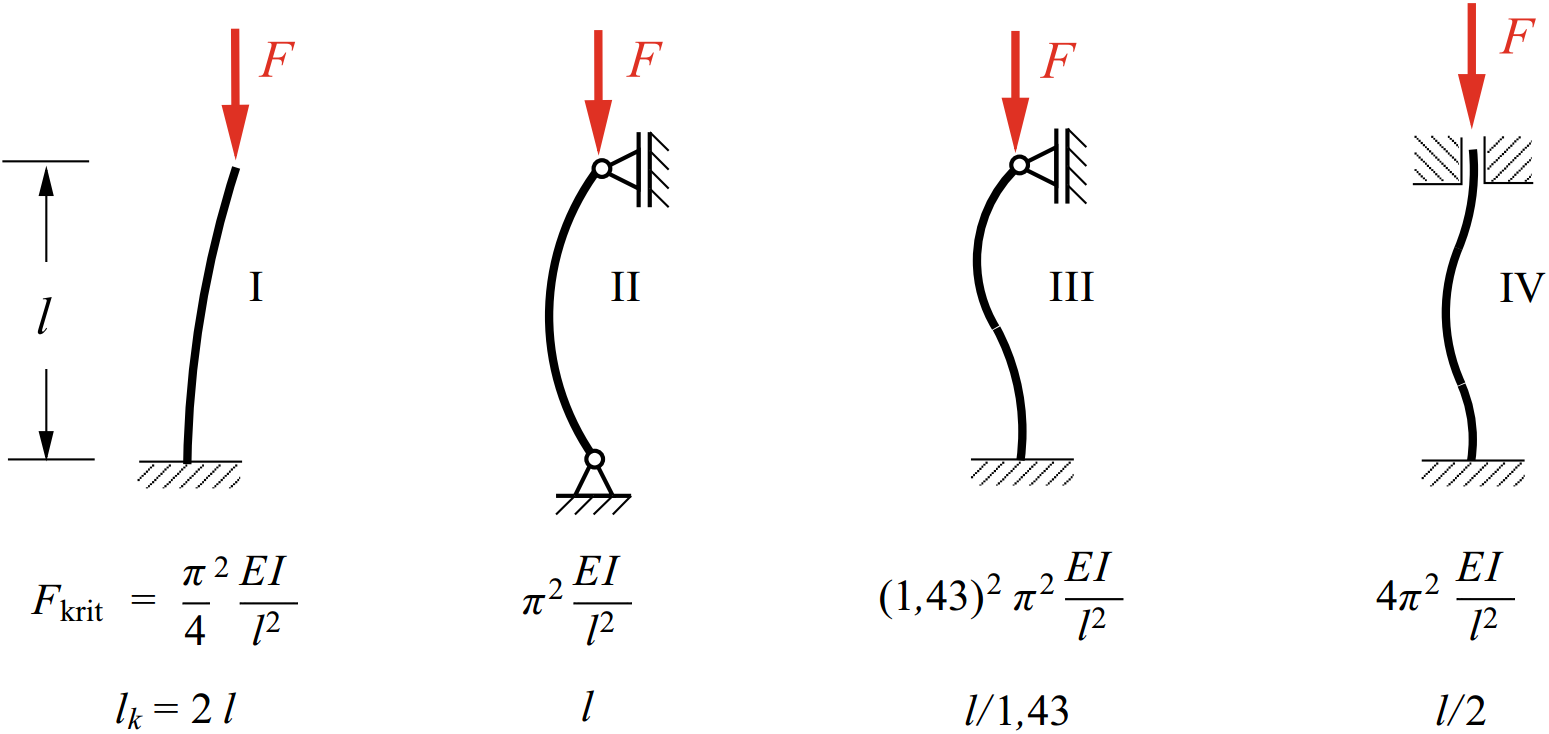
\includegraphics[width=.5\linewidth]{euler.png}
	\end{figure}


	\arraycolsep=2pt
	\def\arraystretch{2}	
	%\rotatebox{90}
	{
		\colorbox{green!60!white!50}
		{
			\begin{equation*}
				%\tag{Flächenträgheitsmomente}
				\begin{array}{|l|*5{>{\displaystyle}c|}}
					\hline 
					\text{Fläche}                                    &               I_y                            &                                        I_z &                                I_{yz} &                                    I_p          & I_{\bar{y}} \\ \hline 
					\text{Rechteck}                                  &   \frac{bh^3}{12}                            &                            \frac{hb^3}{12} &                                     0 & \frac{bh}{12} \left( h^2 + b^2 \right)          & \frac{bh^3}{3} \\ \hline 
	%				Quadrat &  &  &  &  &  \\ \hline   
					\text{\parbox{1.5cm}{Dreieck \underline{BILD}}}    &   \frac{bh^3}{36}                            & \frac{bh}{36}\left( b^2 -ba + a^2 \right)  & -\frac{bh^2}{72}\left( b - 2a \right) & \frac{bh}{36}\left( h^2 + b^2 -ba + a^2 \right) & \frac{bh^3}{12} \\ \hline 
					\text{Kreis}                                     & \frac{\pi R^4}{4}                            &                          \frac{\pi R^4}{4} &                                     0 &                               \frac{\pi R^4}{2} & \frac{5 \pi}{4}R^4 \\ \hline 
					\text{\parbox{1.7cm}{Dünner Kreisring $t\ll R_m$}} &       \pi R^3_m t                            &                                \pi R^3_m t &                                     0 &                                    2\pi R^3_m t & 3\pi R^3_m t \\ \hline 
					\text{Halbkreis}                                 & \frac{R^4}{72 \pi}\left( 9 \pi^2 -64 \right) &                          \frac{\pi R^4}{8} &                                     0 &    \frac{R^4}{36 \pi}\left( 9 \pi^2 -32 \right) & \frac{\pi R^4}{8} \\ \hline 
					\text{Ellipse}                                   & \frac{\pi}{4}ab^3                            &                          \frac{\pi}{4}ba^3 &                                     0 &        \frac{\pi ab}{4}\left( a^2 + b^2 \right) & \frac{5\pi}{4}ab^3 \\ \hline 
				\end{array}
			\end{equation*}
		}
	}

\end{document}


